\documentclass{beamer}% тип документа
% далее идёт преамбула
\usepackage{blindtext}
\usepackage{hypcap}
\usepackage[T2A,T1]{fontenc}
\usepackage[utf8]{inputenc}
\usepackage[russian]{babel}
\usepackage{graphicx}
\usepackage{datetime}
\usepackage{multicol}



\usepackage{caption}
\captionsetup[figure]{font=footnotesize,labelfont=footnotesize}
\begin{document}% начало презентации

\title{Разработка стохастической модели роста филамента в структуре оксидной пленки}
\author{Соловьёв Максим Андреевич}
\date{\today}
\institute{Кафедра физики твердого тела,
Физический факультет,\\
Московский государственный университет имени М.В.Ломоносовва.\\
Научный руководитель: кандидат физико-математических наук\\
    Бажанов Дмитрий Игоревич}



\begin{frame}% первый слайд
\begin{figure}
    \centering
    
\includegraphics[width=60px]{img/ff-sign.png}
\end{figure}
\maketitle
\end{frame}

\begin{frame}{Мемристор}
\begin{multicols}{2}
Мемристор - это пассивный элемент в микроэлектронике, способный изменять свое сопротивление в зависимости от протекающего через него заряда. 
\footnotetext[1]{
    Journal of Vacuum Science and Technology B 29, 01AD03 (2011); doi: 10.1116/1.3521503
}
\begin{figure}
    \centering
    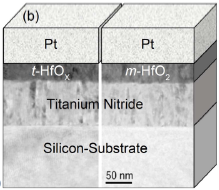
\includegraphics[width=85px]{img/real_memristor.PNG}
    \caption{Пример устройства реального мемристора%
\footnotemark[1]
}
\end{figure}
\columnbreak
    \begin{figure}
        \centering
        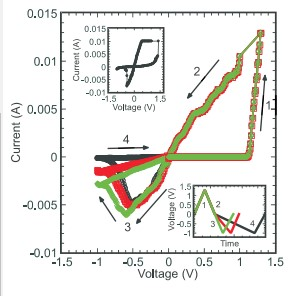
\includegraphics[width=150px]{img/vac_memrister.jpg}
        \caption{ВАХ реального мемристора%
    \footnotemark[1]
    }
    \end{figure}
\end {multicols}
% \footnotetext[2]{G. C. Jegert, “Modeling of Leakage Currents in High-k Dielectrics,” Ph.D. Dissertation, Tech. Univ. Munich,
% Germany, December 2011. }
\end{frame}

\begin{frame}{Мотивация}
\begin{multicols}{2}

% Мемристор может быть использован как синапс в нейроморфных сетях.

% Нейроморфные сети, имеют большой потенциал, так как крайне производительны по сравнению с традиционными реализациями нейронных сетей.

% Соответственно, моделирование мемристоров для определения разных их свойств - значимая область исследования.

Мемристор может быть использован как синапс в нейроморфных сетях.
Соответственно, моделирование разных свойств мемристора имеет большой потенциал.
\columnbreak
    
    \begin{figure}
        \centering
        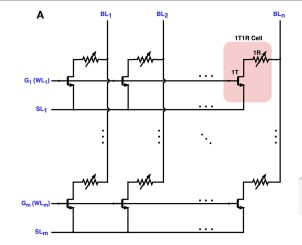
\includegraphics[width=160px]{img/sinaps-memristor-scheme.jpg}
        \caption{Принципиальная схема использования мемристора как синопса в нейроморфной сети%
        \footnotemark[2]
    }
    \end{figure}
    \footnotetext[2]{%
        Guo* Y, Wu H, Gao B and Qian H(2019) Unsupervised Learning on Resistive Memory Array Based Spiking Neural Networks. Front. Neurosci. 13:812. doi: 10.3389/fnins.2019.00812
        }%
\end{multicols}

\end{frame}


%Цель работы - что собираюсь делать и как моделировать
\begin{frame}{Цель работы}

Создание симулятора, позволяющего моделировать мемристор
и протекающие в нем процессы.
\begin{figure}
    \centering
    \includegraphics[width=300px]{schemes/model/model.pdf}
    \caption{
        Принципиальная схема симулятора
}
\end{figure}






\end{frame}

\begin{frame} {Симулируемая структура}
    \begin{itemize}
        \item Структура мемристора - слой диэлектрика, заключенный между парой электродов.
        \item Проводимость мемристора определяется ростом в нем определенной структуры - филаменты (нити).
        \item Филамент в большинстве случаев формируется на неоднородности электрода, поэтому неоднородность добавлена к электроду. \footnotemark[3]
    \end{itemize}

    \begin {multicols} {2}
    \begin{figure}
        \centering
        \includegraphics[height=80px]{schemes/simulator/simulator.pdf}
        %\vspace {11px}
        \caption {Симулируемая структура}
    \end{figure}
    
    \columnbreak

    \begin{figure}
        \centering
        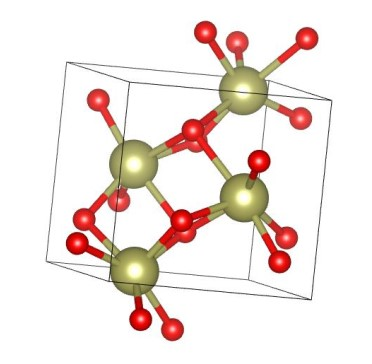
\includegraphics[height=80px]{img/POSCAR.jpg}
        \vspace {12px}
        \caption {Моноклинный \(HfO_2\)}
    \end{figure}

\end{multicols}

\footnotetext[3]{J. Appl. Phys. 125, 234503 (2019); https://doi.org/10.1063/1.5094864}

\end{frame}

\begin{frame} {Реакции}

    \begin {multicols} {2}

    \textbf{Ионные реакции}
    \begin {multicols} {2}
    \begin{figure}
        
        \centering
        \includegraphics[width=60px]{schemes/reacts/R1.pdf}
        \caption{Образование пары ион-вакансия}
        
    \end{figure}

    \columnbreak
    \begin{figure}

        \centering
        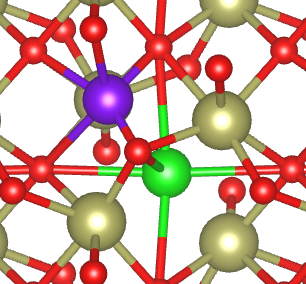
\includegraphics[width=60px]{schemes/reacts/R3.pdf}
        \caption{Рекомбинация пары ион-вакансия}

    \end{figure}

    \end{multicols}

    \begin {multicols} {2}
        
    \begin{figure}

        \centering
        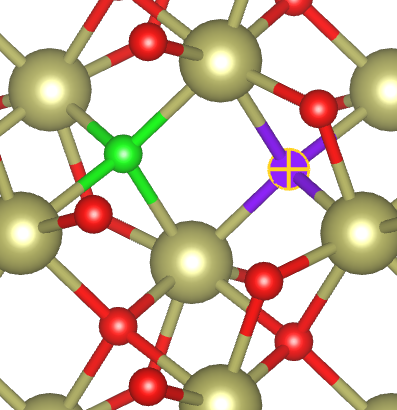
\includegraphics[width=60px]{schemes/reacts/R2.pdf}
        \caption{Перескок иона кисловода между межузельными положениями}

    \end{figure}
    \columnbreak
    \begin{figure}

        \centering
        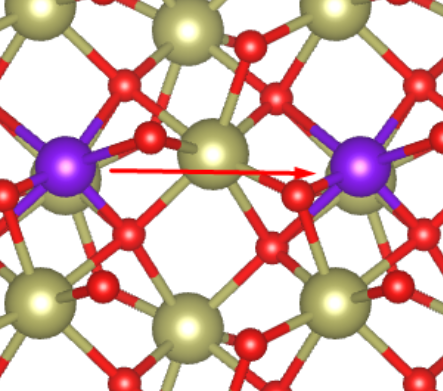
\includegraphics[width=60px]{schemes/reacts/R4.pdf}
        \caption{Перескок иона кислорода мижду узловыми положениями}

    \end{figure}
    \end{multicols}

    \columnbreak

    \textbf{Электронный транспорт и динамика}
    \begin{itemize}
        \item Эффект Шотки
        \item Эмиссия Пуля-Френкеля
        \item Прямое туннелирование
        \item Туннелирование с помощью ловушек (TAT)
    \end{itemize}

    \end{multicols}
\end{frame}

%Слайд с ионными реакциями
% \begin{frame}{Ионные реакции}
%     \begin{figure}

%         \centering
%         \includegraphics[height=40px]{schemes/reacts/types.pdf}

%     \end{figure}




% \end{frame}

% %Слайд для описания электронных реакций
% \begin{frame}{Электронные реакции}



% \end{frame}

%Слайд для формул, описывающих разные ракции

\begin{frame}{Математические основы модели} {Кинетический метод Монте-Карло}

%\textbf{Кинетический метод Монте-Карло}


В системе заданы N реакций с частотами: $\nu_i$.\
За каждый КМК шаг выбирается 1 реакция:
\[S_i = \sum_{j=1}^{i}{\nu_j}\]
\[R \in U[0,S_N)\]
\[S_i \le R < S_{i+1}\] 

\begin{figure}
    \centering
    \includegraphics[width=150px]{schemes/KMK_math/kmk_math.pdf}
\end{figure}

$\tau = \frac{1}{S_N}$ - время, за которое происходит этот шаг КМК.

\end{frame}

% Для ионных реакций:

\begin{frame}{Математические основы модели} {Частоты реакций}

    \small

    Напряжение в любой точке находится как:

    \[U = \frac{l\cdot U_{cond}}{D}+U_{evald}\],

    где \(U_{cond}\) - Напряжение между электродов, \(l\) - расстояние до положительного электрода, \(D\) - расстояние между электродами, а \(U_{evald}\) - периодический потенциал, рассчитанный с помощью метода Эвальда.

    Частоты протекания ионных реакций находятся по формуле:

    \[\nu = \nu _0 \cdot
    \exp{(-\frac{E-\gamma \Delta q \Delta U}{k_bT})} \cdot
    \exp{(-\frac{\Delta a}{a})}
    \],

    где T - температура,
    \(k_b\) - постоянная больцмана,
    E - барьер реакции,
    \(\Delta q\) - переносимый заряд,
    \(\Delta a\) - расстояние, на которое заряд переносится,
    \(\Delta U\) - напряжение между начальным и конечным положением,
    \(\nu_0\)  - базовая частота реакции,
    \(a\) - Длина локализации,
    \(\gamma\) - вклад поляризации связей в локальное электрическое поле.
    

    
\end{frame}


%Используемые в модели константы
\begin{frame}{Параметры и константы}
    \begin{table}
        \begin{tabular}{llc}
          Параметр & Величина\\ 
          Базовая частота (\(\nu _0\)) &
          \(10^{-13} s^{-1}\) \\
          \(\gamma\) & 4.0 \\
        \end{tabular}
        \caption{Базовые константы}
      \end{table}

      \begin{table}
        \begin{tabular}{llc}
          Реакция & Барьер (эВ) \\ 
          R1 &  \(6.4\) \\
          R2 &  \(1.4\) \\
          R3 &  \(0.8\) \\
          R4 &  \(4.1\) \\
          E1 &  \(0.3\) \\
          E2 &  \(0.3\) \\
          E3 &  \(0.3\) \\
        \end{tabular}
        \caption{Барьеры реакций}
      \end{table}


\end{frame}

% \begin{frame} {Найденные барьеры}

%     \begin {multicols}

%     \begin{figure}

%         \centering
%         \includegraphics[width=100px]{img/barrier/R1}
%         \caption{Барьер R1}

%     \end{figure}

%     \begin{figure}

%         \centering
%         \includegraphics[width=100px]{img/barrier/R1}
%         \caption{Барьер R2}

%     \end{figure}
%     \columndreak

%     \begin{figure}

%         \centering
%         \includegraphics[width=100px]{img/barrier/R1}
%         \caption{Барьер R3}

%     \end{figure}

%     \begin{figure}

%         \centering
%         \includegraphics[width=100px]{img/barrier/R1}
%         \caption{Барьер R4}

%     \end{figure}
%     \end{multicols}
    
% \end{frame}

%Слайд с видом всей смоделированной структуры

% \begin{frame}{Смоделированная структура}
%     \begin{figure}
%         \centering
%         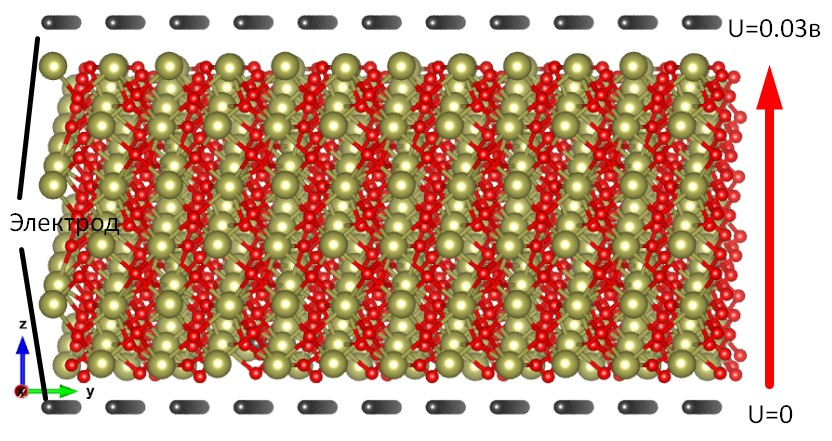
\includegraphics[width=300px]{img/model-result-v3.jpg}
%     \end{figure}

% \end{frame}

%На этом слайде будут/ет картинка с полученным филаментом.
\begin{frame}{Смоделированная структура}{}

В результате работы удалось смоделировать рост филамента в мемристоре.

\begin {multicols} {2}

\begin{figure}
    \centering
    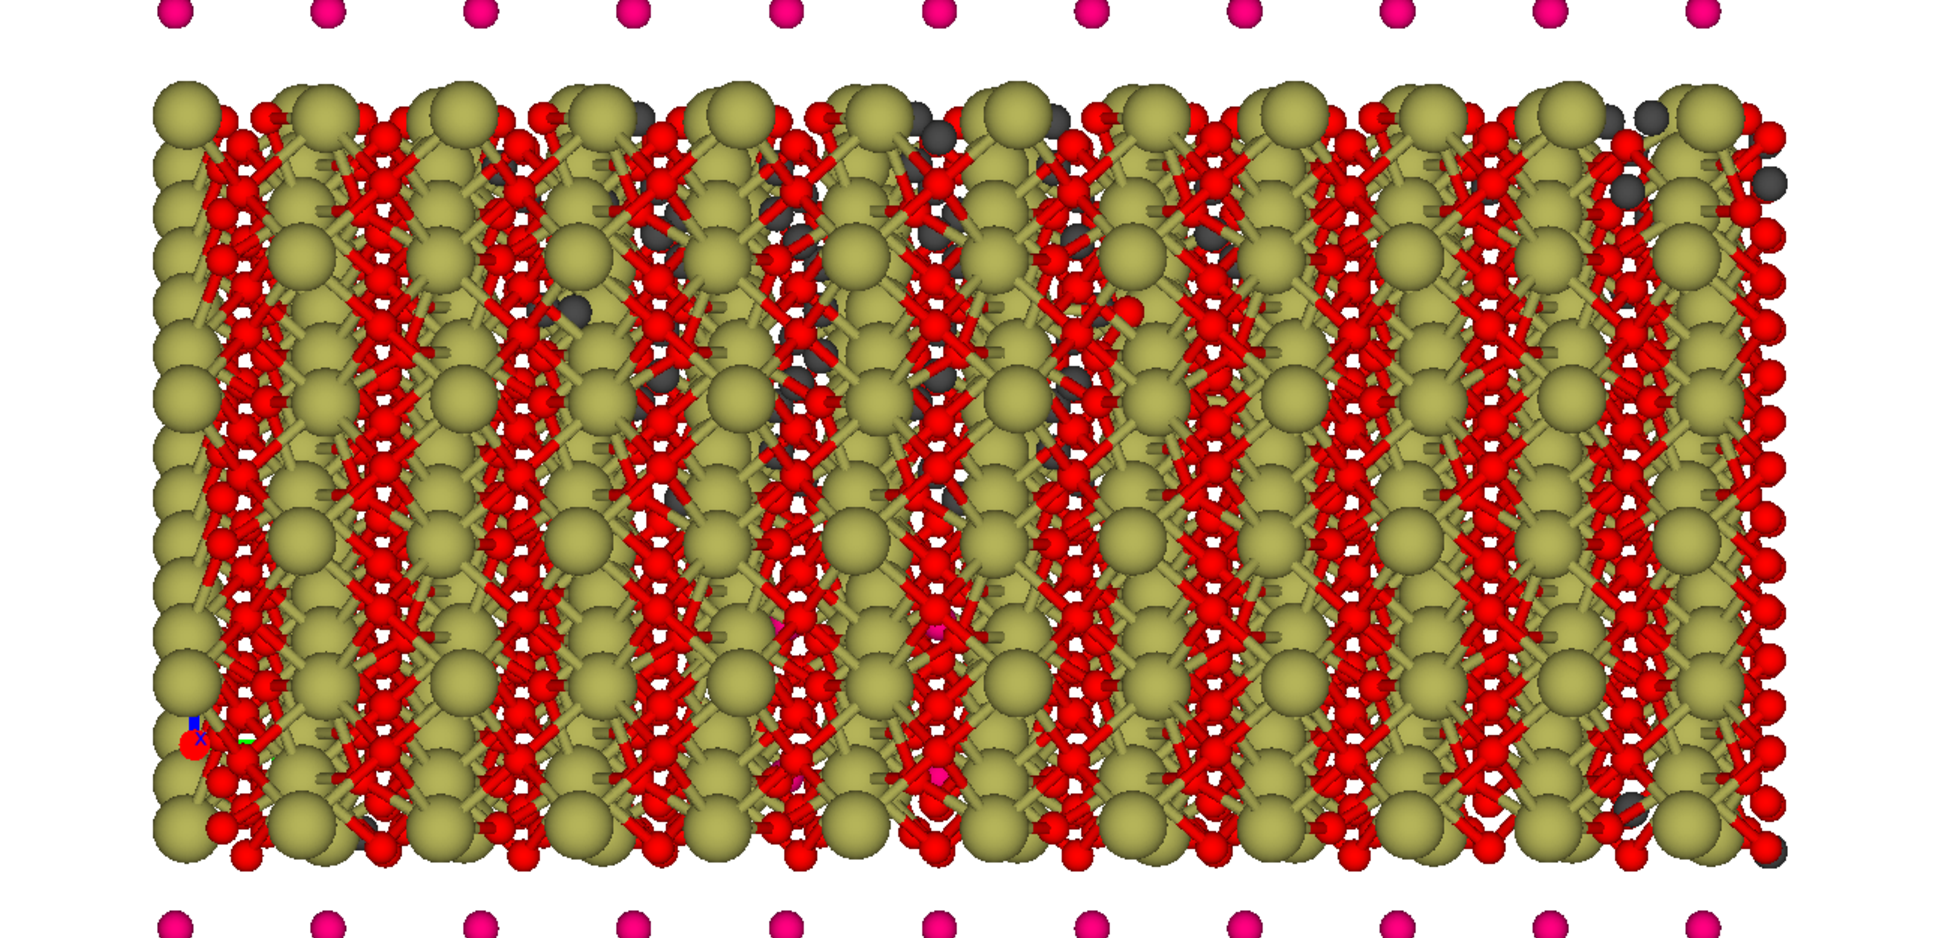
\includegraphics[height=80px]{img/11000_full_ex.pdf}
    \caption{Полная смоделированная структура.
    }
\end{figure}
\columnbreak

\begin{figure}
    \centering
    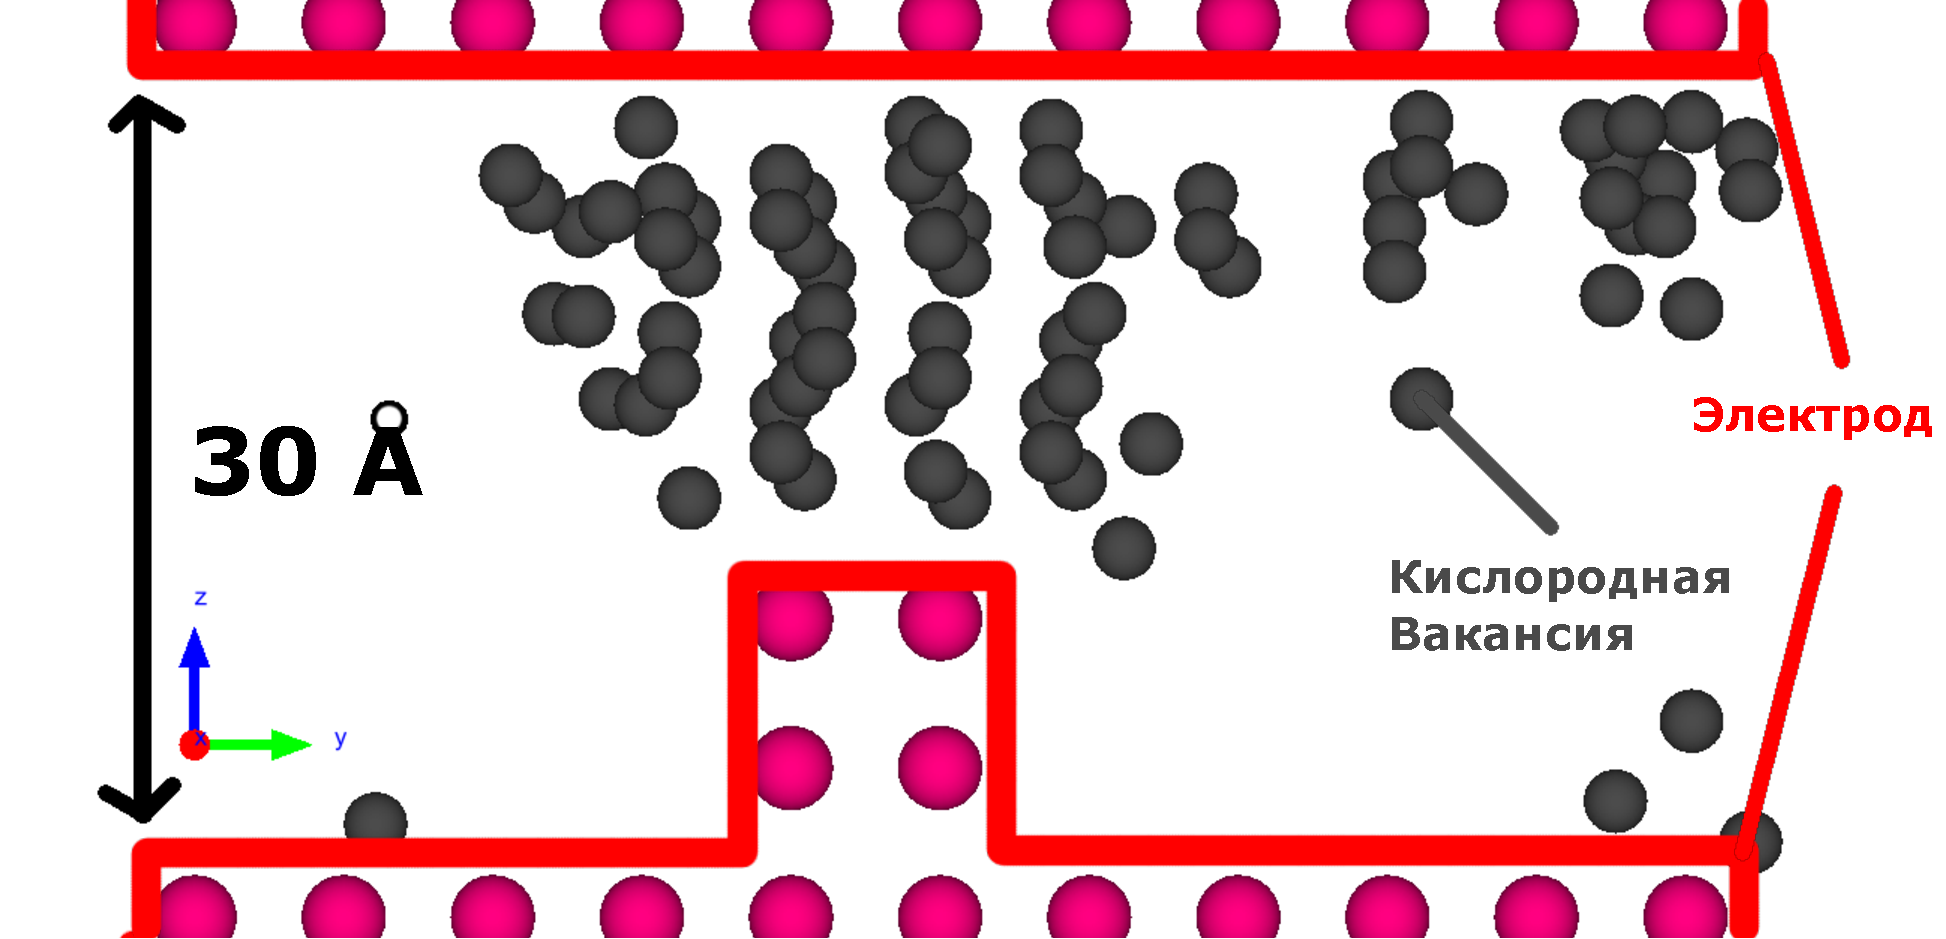
\includegraphics[height=80px]{img/11000_ex.pdf}
    \caption{Филамент при напряжении 0.9В между электродами.
    Фиолетовые шарики - атомы электрода.
    Серые - кислородные вакансии.
    Расстояние между электродами 30 Ангстрем.
    }
\end{figure}

\end{multicols}
\end{frame}

%Есть надежда получить реакции set-reset и показать их оттельно, но пока еще нет.
\begin{frame}{ВАХ смоделированной системы}
    Была проведена симуляция системы при разных напряжениях и начальных условиях.
    Это позволило получить Вольт-амперную характеристику.
    \begin {multicols}{2}
        \begin{figure}
            \centering
            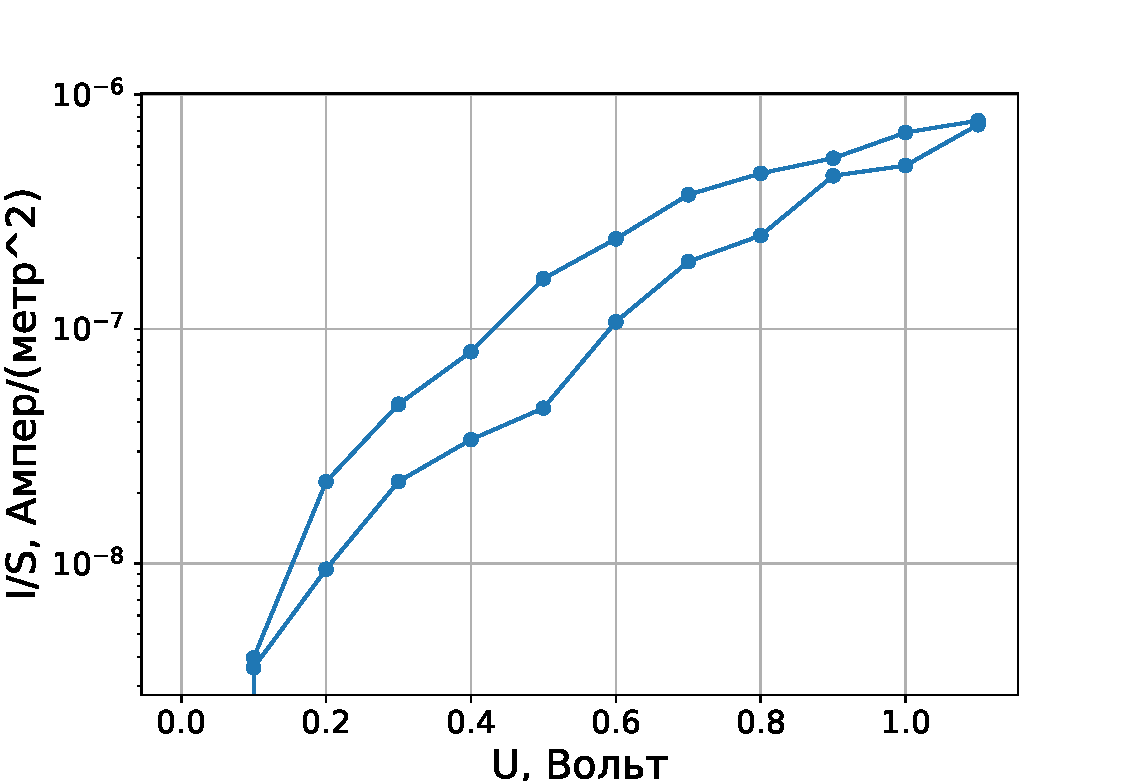
\includegraphics[width=170px]{img/SET.pdf}
            \caption {Процесс SET}
        \end{figure}
        \columnbreak
        \begin{figure}
            \centering
            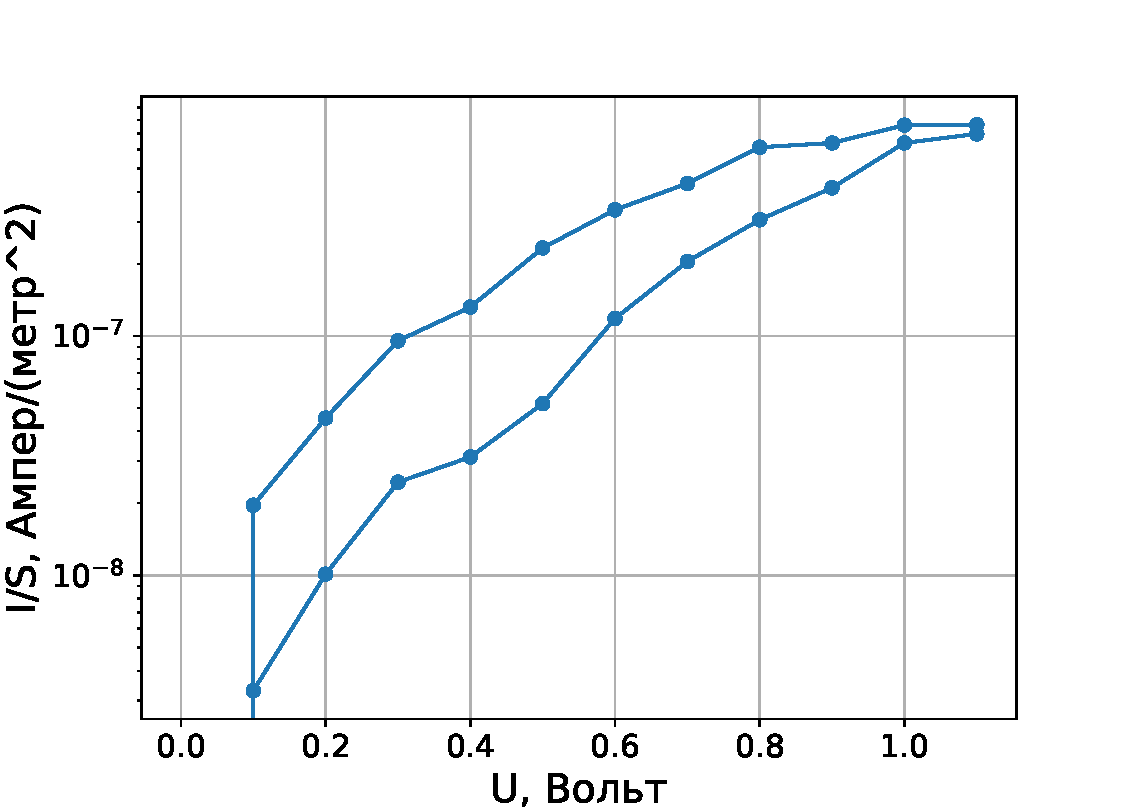
\includegraphics[width=170px]{img/RESET.pdf}
            \caption {Процесс RESET}
        \end{figure}   
    \end{multicols}

\end{frame}

%Слайд с обобщенными результатами
\begin{frame}{Результаты}

\begin{list}{*}{}
    \item  Разработана и реализована модель для симуляции роста филаментарных структур с использованием кинетического метода Монте-Карло
    \item  С использование теории функционала плотности выполнены рассчеты для параметризации процессов.
    \item  Работа модели была проверена, и на её основании было получены и продемонстрировано образование филаментарной структуры при наличии внешнего поля.
\end{list}
\end{frame}
%Слайд с тем, что еще можно сделать
\begin{frame}{Планы}

\begin{list}{*}{}
    \item  Учет сложной структуры интерфейса на границе Оксид-Электрод
    \item  Рассмотрение разных форм электрода.
    \item  Рассмотрение разных веществ в качестве электрода/диэлектрика.
    \item  Изучение вклада от разных способов течения тока в общий ток.
\end{list}



\end{frame}

\begin{frame}[plain]
\vfill
\centerline{Спасибо за внимание!}
\vfill\vfill
\end{frame}

%Секретный слайд
%Секретный - потому, что пока показывать во время основной презентации не планирую
\begin{frame}{Set-Reset в мемристоре}
    \begin{figure}
        \centering
        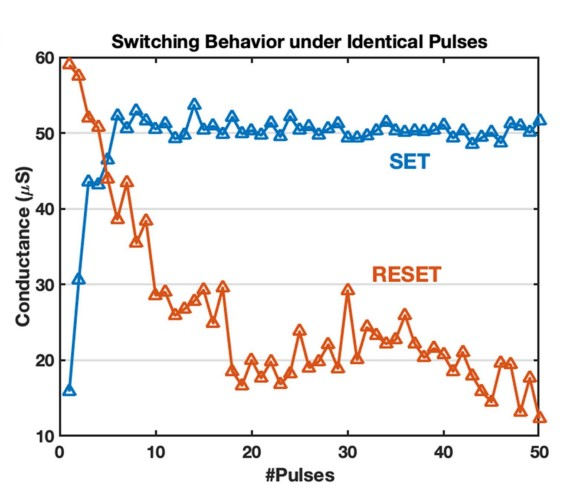
\includegraphics[width=180px]{img/memristor-set-reset.jpg}
        \caption{Set-reset в мемристоре%
    \footnote{%
    Guo Y, Wu H, Gao B and Qian H(2019) Unsupervised Learning on Resistive Memory Array Based Spiking Neural Networks. Front. Neurosci. 13:812. doi: 10.3389/fnins.2019.00812
    }%
  }
    \end{figure}
\end{frame}


\end{document}